\chapter{考察}
\label{chapter:consideration}

\section{MPTCPを有効活用するトポロジーに関する考察}

Fig.\ref{fig:multi-homing}にk-MHFTを示す. 
k-aryマルチホーミングトポロジーはFatTreeと同様に, k個のポッドから構成されおり, 
一つのポッドで$k/2, k^2/4$それぞれaggregatorスイッチとedgeスイッチを持つ. 
aggregatorスイッチとedgeスイッチではそれぞれ,
$k/2$のノードと上位レイヤーのスイッチ1つに接続し, 計$k/2+1$ポートが必要である. 
また, coreスイッチは$k/2$台の$k/2$ポートスイッチが必要である. 
さらに, MHFTは$k^3/4$までのノードを持つことができ, $k/2$のインタフェースが必要であるとする. 
この時, $k/2$本の経路が, 物理的に等価なコストの経路数となる. 


\begin{table}[t]
    \begin{center}
    \begin{tabular}{c|c|c}
    k-ary & Number & Port/Interface \\ \hline
    core & $k/2$ & $k/2$ \\ \hline
    aggregator & $k^2/2$ & $k / 2 + 1$ \\ \hline
    edge & $k^3 / 4$ & $k / 2 + 1$ \\ \hline
    node & $k^3 / 4$ & $k / 2$ \\
    \hline
    \end{tabular}
    \caption{Multi-homing FatTree constitution}
    \label{table:mhft_constitution}
    \end{center}
\end{table}


ネットワーク帯域の効率的な利用を目指す取り組みとして, 様々なデータセンターネットワークトポロジーが提案されている. 
提案されているトポロジーは, 複数の等コストな経路がある冗長性を持たせた構成になっており, そうした経路を有効活用する手段としてMPTCPがある. 
$\S$\ref{sec:traffic}に示したように, MPTCPを用いることで,
将来の広帯域化により発生すると予想されているノード側のボトルネックについても, 解決することができると期待されており,
デュアルホーミングを活用したトポロジーも提案されている\cite{improving}. 
具体的には, 今日のサーバでは一般的である複数のNICに対してMPTCPを利用するということである. 
そこで本研究では, エンドノードの持つ複数のNICを有効活用するためのトポロジーとして, MHFTを提案した. 
しかし, 今日の巨大なクラスターを持つデータセンターの設計には, 性能の優位さだけではなく構築に掛かるコストについても考慮しなければならない. 
そこで, MHFT構築に掛かるコストについて, 保有できるエンドノードの台数とともに検討を行う. 
検討には, エッジ部分でのスイッチとして48ポート1ギガビットスイッチ(\$7000)とアグリゲーション,
コア部分でのスイッチとして128ポート10ギガビットスイッチを用いて構成する際のコストを検討する\cite{fattree}.
なお, 配線ケーブルのコストは考慮しないこととする. 

Fig.\ref{fig:MHFT_cost}に, 保有できるホストの数とトポロジー形成に掛かる費用の関係を示す. 
例えば, 20000ホストに対するスイッチ機器を考えたとき, Fattreeトポロジーでは, 1152台のedgeスイッチ,
1152台のAggregationスイッチ, 576台のcoreスイッチによって構成することができ, かかる費用は約\$1217Mである. 
一方MHFTにおいて20000ホストを保有するトポロジーを構築しようとすると,  27648台のedgeスイッチ,
1152台のAggregationスイッチ, 24台のcoreスイッチによって構成することができ, かかる費用は約\$1016Mである. 

このように, MHFTではコスト面では有効であると言える.
しかし, FatTreeに比べ, 等コストな経路の数は少なくなっており, 通信負荷分散の可能性としてはFatTreeの方が潜在している. 


\begin{figure}[t]
    \begin{center}
    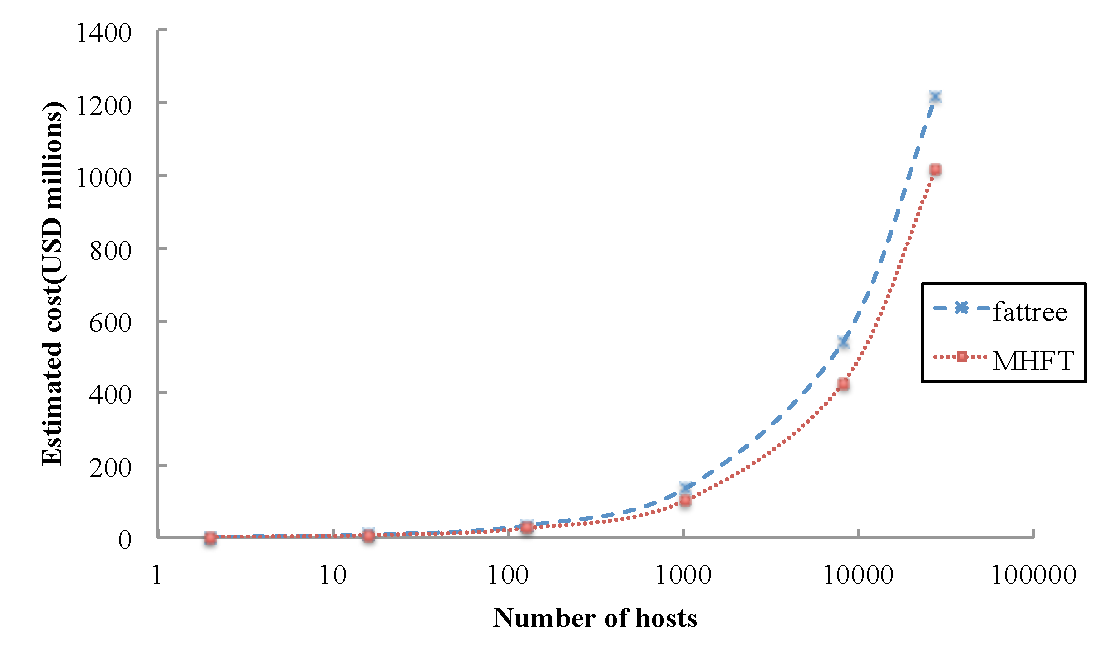
\includegraphics[autoebb, width=250pt]{./img/mhft_cost.pdf}
    \caption{Current cost estimation vs. maximum possible number of hosts}
    %\ecaption{The control loop in DCTCP}
    \label{fig:MHFT_cost}
    \end{center}
\end{figure}


\section{レーンモデルに対する考察}
SL2LL1やSL2LL2の結果を示す. 

\section{リンクコストベースの切替手法のパラメータに関する考察}
リンクコストのパラメータとして$t_{deadline}, \alpha \sim \delta$があり, 今回の評価の際にはべき乗部分にあたる$\beta,
\delta$については固定して評価を行った. 
これはリンクコスト計算においてべき乗の影響は大きく, 一方を大きくするとその項が支配的に作用するためである. 
リンクコストの定義の意味を考慮して, $\beta=\delta$とそれぞれの項の次元をを揃えることが望ましいと考える. 

$t_{deadline}$については, 対象となるアプリケーションが最低限満たすべき通信時間の値を設定するべきである. 
一般に, 近年のデータセンターにおける並列分散処理アプリケーションでは, 300ms以内に通信を終えるべきであるとしており, 評価実験においてもその値に従った. 

$\alpha, \gamma$については, 通信状況に対し機敏に反応させたければ, $\alpha$を大きく, $\gamma$を小さく設定するべきである. 
しかし, それらを極端な値に設定すると, 一方のレーンに通信が偏る可能性がある. 
また, しきい値を満たすショートフローの割合を大きくするには, $t_{deadline}$を本来のしきい値より小さくし, $gamma$を大きく,
$\alpha$を小さくすれば良い. 
これにより, SLへの負荷を減らすことができ, SLを良好な状態に保つことができ,
アプリケーション要求を満たすフローの割合を大きくすることができると考えられる. 
最適なパラメータについては, そのネットワークが持つレーン数や, アプリケーションによって決まると考えられる. 


\section{MPTCPアドレスペアの問題に関する考察}
現状のMPTCPの実装上, サブフローを形成する際での信負荷の分散が有効に働かない問題がある. 
今, Fig.\ref{fig:mptcp_pair}のような複数インタフェースを持つエンドノード間の通信を考える. 
この時, 現状のMPTCP実装では, 互いのアドレスを交換(ADD\_ADDRESS)しあった後,
フルメッシュな組み合わせのIPアドレスでサブフローが形成される. 
具体的には, 1つのTCPコネクション($F1{src:10.1.0.1, dst:10.2.0.1}$)と3つのサブフロー($F2{src:10.1.0.1,
dst:10.2.1.1}, F3{src:10.1.1.1, dst:10.2.0.1}, F4{src:10.1.1.1,
dst:10.2.1.1}$)が形成される. 
静的なIPベースのルーティングを想定した環境において, フロー$F1$はサーバ側へのデータパケット通信に対して$Data:S1-S2-S4$,
クライアント側へのACKパケット通信に対しては$ACK:S1-S2-S4$の経路をそれぞれ用いる. 
同様に, フロー$F2$は$Data:S1-S2-S4, ACK:S1-S3-S4$, フロー$F3$は, $Data:S1-S3-S4,
ACK:S1-S2-S4$, フロー$F4$は, $Data:S1-S3-S4, ACK:S1-S3-S4$の経路をそれぞれ通る. 
基本的にデータパケット通信の方がデータサイズもパケットの数も多いため, キューイング遅延がより起こりやすい通信であり, 例えばフロー$F1$to
$F2$では異なるサブフローにも関わらず, Dataパケットは同一の経路を通る. 
また, MPTCPはそれぞれのフローを同一のものとして輻輳制御を行うため, 経路によってはトラフィックが偏る可能性があり, 有効的な経路利用を実現できない. 

今回のような複数の経路を持つネットワーク環境において, 通信不可の分散の点から理想的なサブフローの形成は,
1つのTCPコネクション(${src:10.1.0.1, dst:10.2.0.1}$)と1つのサブフロー(${src:10.1.1.1,
dst:10.2.1.1}$)が形成されることである. 
すなわち, 1インタフェース1サブフローの原則による, 重複のないIPアドレスのペアを形成することで, 最適なトラフィック負荷の分散を実現できる. 
そのため, 本提案手法の実装にあたり, 今のMPTCP実装に対して変更を加えた. 


\begin{figure}[t]
    \begin{center}
    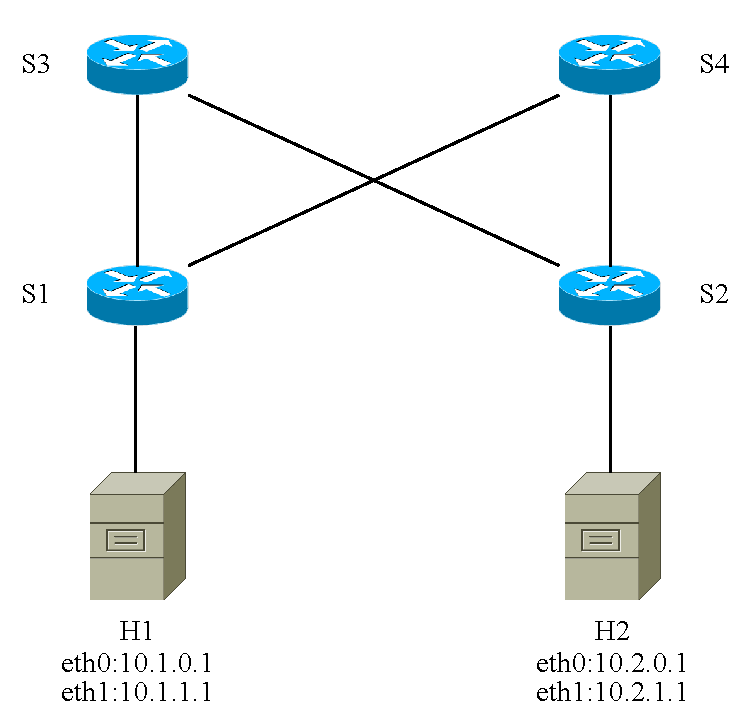
\includegraphics[autoebb, width=250pt]{./img/pair_problem.pdf}
    \caption{Techinical problem of creating subflow without complete paired IP
    addressses}
    %\ecaption{The control loop in DCTCP}
    \label{fig:mptcp_pair}
    \end{center}
\end{figure}

\section{Incast問題に対する考察}
データセンターが抱える性能障害の一つにIncast問題がある. 
これは, 一つのインタフェースに大量のショートフローが同時に集中することにより遅延が生じるという, データセンターでの並列分散処理が生み出す特有の問題である. 
今のMPTCP実装では, サイズの小さい通信には複数経路を用いずに一つの経路だけで通信が完了するため, 今回の提案手法のような経路切替手法は有効に働かない. 
例えば, エンドノード間の通信経路が3本存在している時には, SLに2経路, LLに1経路割り当て,
ラウンドロビンやハッシュベースを用いた負荷分散手法が有効であると考える. 
このような従来のECMPによるアプローチと比べ, レーンモデルによるフローの区別を行うことで, ショートフローに対してのみロードバランスすれば良いため,
Fig.\ref{fig:repflow_scenario}のような性能障害が起きないと考える. 

実際。。。(グラフを示す)

